\documentclass[a4paper,12pt]{article}

% 导言区
\usepackage{titlesec}
\usepackage{lipsum} % 示例用,可以删除
\usepackage{geometry}
\usepackage{setspace}
\usepackage{amsmath} % 用于数学公式
\usepackage{graphicx} % 用于插入图片
\usepackage{float}
\usepackage{lipsum} % 用于生成虚拟文本
\usepackage{ctex} % 导入 ctex 包以支持中文
\usepackage{xeCJK}
\usepackage{titlesec} % 导入 titlesec 包以定制标题样式
\usepackage{fontspec} % 用于设置中文字体
\usepackage{amsfonts}
\usepackage{amsmath} % 提供 \text 和 \tanh 命令
\usepackage{bm}      % 提供 \bm 命令用于粗体

% 目录设置
\usepackage[nottoc,notlot,notlof]{tocbibind}
\usepackage{enumitem}
% 页面设置
\geometry{margin=1in}

% 标题设置
\titleformat{\section}{\normalfont\Large\bfseries}{\thesection}{1em}{}
\titleformat{\subsection}{\normalfont\large\bfseries}{\thesubsection}{1em}{}
\titleformat{\subsubsection}{\normalfont\normalsize\bfseries}{\thesubsubsection}{1em}{}

% 行间距设置
\onehalfspacing

% 文档信息
\title{商业模式设计}
\author{需求不寄小分队}
\date{\today}

\begin{document}

\maketitle

% 添加目录
\tableofcontents

\section{团队成员}
\begin{itemize}
    \item 211250124 程智镝
    \item 211250122 刘辉
    \item 211250159 陈凌
    \item 211250158 李忠信
\end{itemize}

\subsection{度量数值}
    
\section{文档简介}
我们按照商业模式画布,使用教材讲述的六种设计方法,对之前的分析进行了梳理与完善。较之之前的
分析结果,更加清楚地完善了产品的价值追求。明确了我们产品的创意方向,与较之其他产品的关键性
创意。摒弃了之前一些大而空的产品构思,分析结果更加具体,明确。

\section{客户洞察}
\subsection{高校教师}
作为一款大众会议虚拟软件,我们意识到在疫情过后,学校师生对会议软件的需求量大幅增加。因此,我们希望打造一个专门服务于教学领域的教育软件。除了提供基本的会议功能外,我们还致力于为教师和学生提供更专业、更便捷的服务,例如在线答题、定期会议、讨论小组等功能,以模拟线下教学的模式。我们的目标是让教师和学生在使用我们的软件时能够体验到线下教学的特色,同时享受线上会议的高效便捷,从而实现教学的智能化与便利化。

下图展示了一个高校老师小陈由于疫情原因无法线下上课,教学问题成为他急需解决的问题。我们希望通过我们的软件,能够帮助像小陈老师这样的教师解决线上教学所面临的挑战,提升他们的教学效率和质量。
\begin{figure}[h]
    \centering
    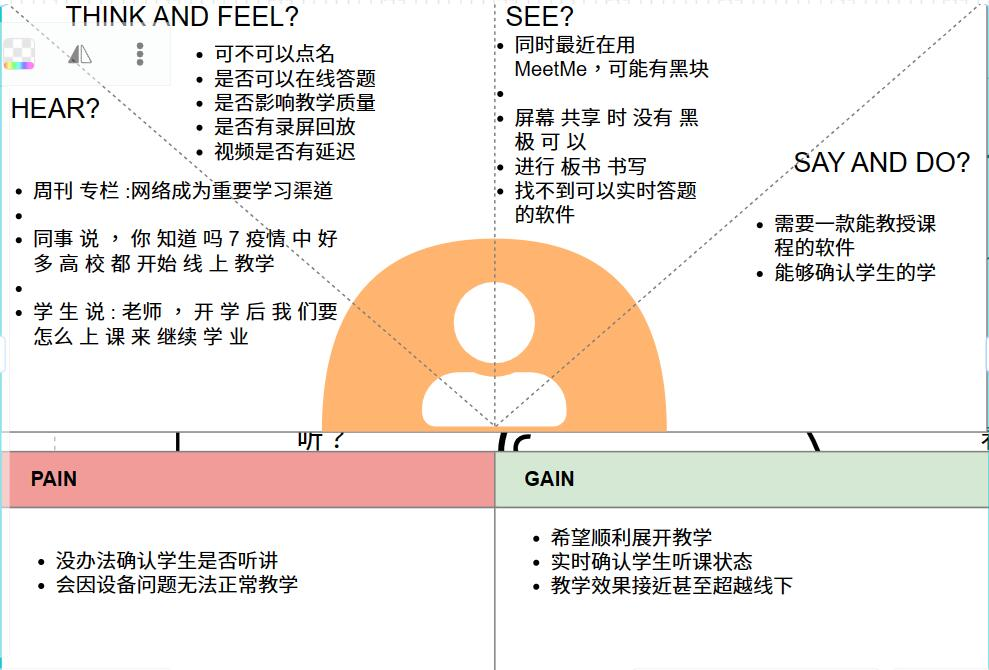
\includegraphics[width=0.8\textwidth]{高校移情图.jpg}
    \caption{Your caption}
\end{figure}
\clearpage


\subsection{企业主管}
在企业会议中,我们的软件支持多人共享屏幕和远程设备操作,并且能够将会议文件安全地保存在云端。对于重要的会议,特别是涉及商业机密和重要客户资料的高层级会议,我们提供了加密算法来保护数据传输安全,以防止黑客入侵和信息窃取。

对于跨国企业的企业主管,我们的软件可以满足其与各国小组成员或支持业务部门进行安全交流与会议的需求。在跨国交流中,可能涉及公司的敏感信息和机密数据,因此我们提供了可靠且安全的软件来保障交流的安全性。

通过我们的软件,企业主管可以放心进行跨国远程交流,而无需担心信息安全问题。我们致力于提供高质量、安全可靠的会议解决方案,以满足企业在全球范围内的远程会议需求。
\begin{figure}[h]
    \centering
    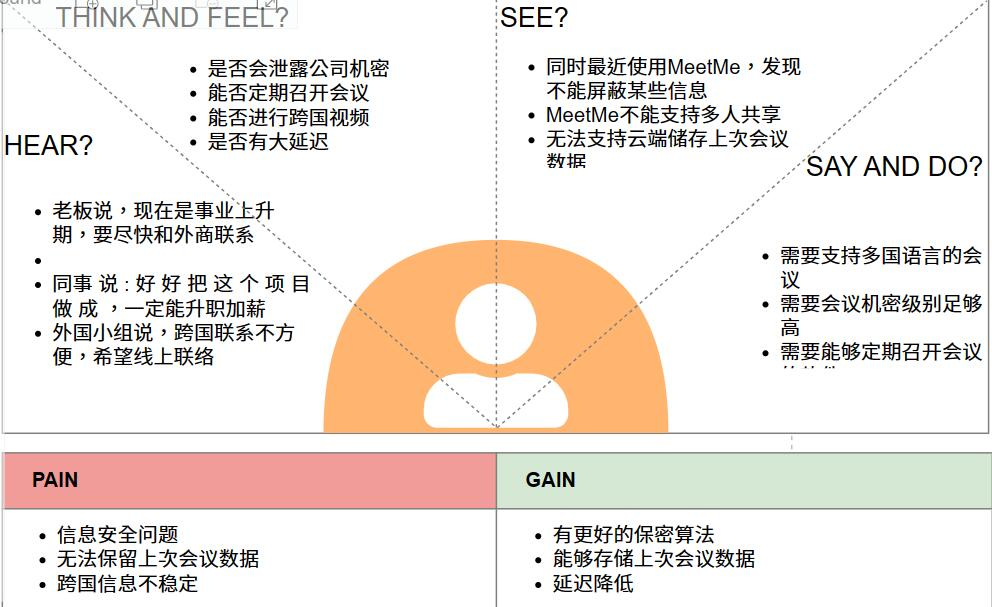
\includegraphics[width=0.8\textwidth]{企业移情图.jpg}
    \caption{Your caption}
\end{figure}
\clearpage


\subsection{电影爱好者}
本平台通过向大量的流媒体公司购买公开放映的版权,获得音乐和视频的播放权。我们在会议中添加了娱乐功能,让会议不再局限于严肃的教学和办公,而是为大家提供一个娱乐和放松的空间。在我们的会议平台上,与会者可以一起阅读书籍、共同观赏电影、共享音乐等。

阿水是电影同好会的成员,他和他的社团成员因为地理位置不同,无法随时聚在一起。因此,他正在寻找一个便捷的方式,在周末与社团成员一起观影。我们的平台正是为了满足像阿水这样的用户需求,让他们能够通过我们的会议平台,轻松地一起观赏电影,即使身处不同的地理位置也能共享同样的娱乐体验。
\begin{figure}[h]
    \centering
    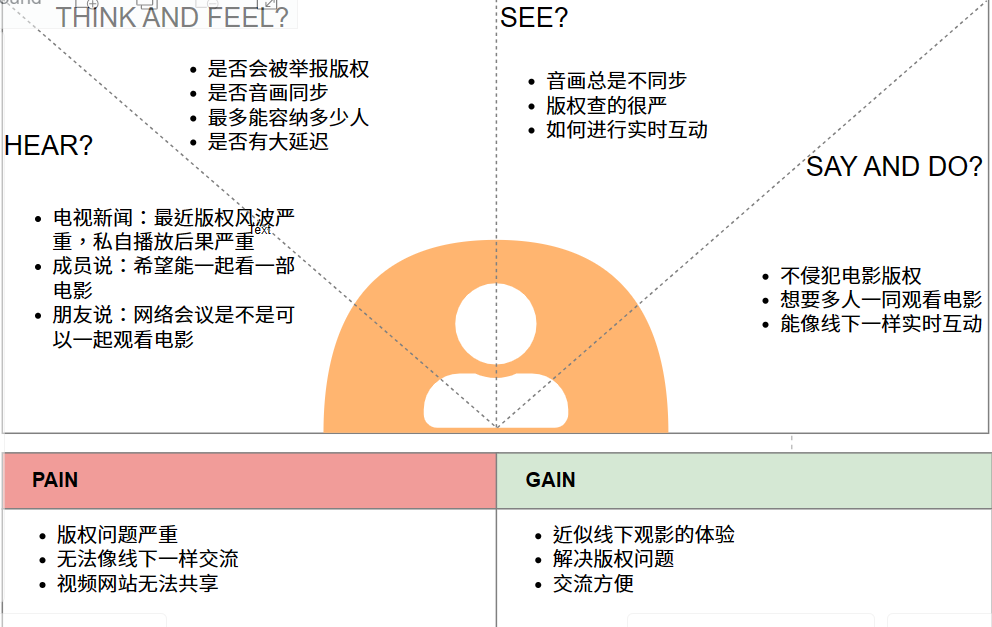
\includegraphics[width=0.8\textwidth]{电影爱好者移情图.png}
    \caption{Your caption}
\end{figure}
\clearpage

\section{构思}
\subsection{从财务驱动的角度出发}
如果我们在产品上线的初期通过向云服务商购买云服务器资源的方式来缩减向用户提供云服务的成本会怎么样?

自行进行云服务器的搭建这一项活动本身是重资产的,在产品上线的初期,我们可能是没有足够的资金来进行服务器的购置和云服务器的构建的。尽管有人会说,我们可以像ofo和瑞幸一样,只要饼画的足够的好,就能吸引足够的融资来实现重资产的想法。这样的想法是太过于幼稚的,要知道,我们自行构建云服务器的想法在营收上就不是太为乐观的,就算是可以像阿里一样将闲置的计算资源开发成提供阿里云的方式来带来营收,其回报率在短时间内是较低的,很容易就会像ofo一样在最后不堪重负,连押金都退不回来;除此之外,技术的限制才是最大的问题,高昂的开发成本和维护成本对我们这样刚开始运营的公司的压力是巨大的,很有可能就是适得其反的行为。因此,在我们产品上线的初期,我们更倾向于与云服务商合作,并向其购买云服务器资源来为我们的用户提供云服务的方式。这样的成本是相对可控并且较为低廉的,可以在初期尽可能的帮我们缩减成本,以维持我们更好的商务运营。

\subsection{从客户驱动的角度出发}
如果客户觉得我们的界面交互不够人性化,吐槽或提出建议会怎么样?

首先,我们的产品是有一个用户可以向我们反馈问题的“社区”的,用户任何吐槽或者建议都可以通过“社区”或者问卷的形式向我们进行反馈。我们会对用户的反馈采用聚类的技术来进行共性问题的筛选。对于对我们人性化功能的建议在通过我们产品部门的调整和优化之后,会提交给技术部门实现,然后上线测试版本,同时再通过问卷的形式听取测试版本使用者的反馈,来进行取舍和再优化。对于一些可能是部分受众所青睐的交互方式,我们会设计成可选项,方便用户进行自定义,最终达到每个用户都能拥有最舒适的体验感,达到近乎于“私人订制”的境界。

\subsection{从供给驱动和财务驱动的双重角度出发}
如果我们产品对基础使用进行免费,为一些想要拥有更为个性化设置、更长会议时间、更多最大参会人数、更大的云存储空间等的用户提供收取一定费用的VIP服务会怎么样?

针对不同的客户群体提供不同的服务,这是有利于我们吸引不同样的客户群体的。对于产品的基础使用提供免费的服务,而且基础的使用也能给客户较为舒适的使用体验,这在产品发行的前期是十分有利于我们口碑的积累的,拥有足够优秀的口碑可以帮助我们在这个赛道拥有自己的一席之地,从而拥有持续发展生存的基础。同时我们会提供一定的增值服务,为一些拥有对更为个性化设置、更长会议时间、更多最大参会人数、更大的云存储空间的需求的用户,我们会为其提供更多的资源,同时收取一定的服务费用,从而成为我们的一项收入来源,帮助我们更好的持续发展。

\subsection{从客户驱动的角度出发}
如果客户在使用过程中对指定的用户群有频繁会议连接的需求会怎么样?

很多用户在使用过程中会对指定的用户群有频繁会议连接的需求。如果还需要通过其他渠道来分享会议链接,会给客户带来额外的工作量,很有可能会引起客户对”繁琐“流程的反感。因此,面对上述的问题,我们的产品会提供简洁且有针对性的社交系统,客户可以通过我们的社交系统建立自己的联络网、通讯录,然后就可以在我们的社交系统内直接“一键”向指定的用户分享会议邀请链接,指定用户就可在我们的社交网络中进行接受邀请或者拒绝邀请的操作,从而形成用户之间的“互联”,满足客户在使用过程中对指定的用户有频繁会议连接的需求,大幅降低客户之间交流的成本,提高工作的效率。

\subsection{从资源供给的角度出发}
如果我们的视频软件平台使用自己的云服务会怎么样?

对于视频会议软件,云服务的可靠性和安全性的要求是非常高的。如果我们全部使用自己的云服务器进行服务,为了维持应用级容灾的成本会非常恐怖。所以我们倾向于将软件开发初期的云服务委托给外部的第三方服务商,使用它们已经成熟的技术对服务的稳定性进行保证。保证核心用户数据以及私人的隐私信息在我们自己的服务器集群中,在软件达到一定的规模之后可以使用自己的云服务进行一定的替换,对数据安全性能够提更高的保障。

\subsection{从客户驱动角度出发}
如果软件平台没有客户想要的影视作品,我们根据客户需求引入会怎么样?

对于平台内缺少的影视作品,用户可以提出引进需求,每隔 1-2 周平台进行一次统计,对需求量最大的前几名予以引入。从客户关系角度出发,能够按用户的需求引入影片,无疑 会让我们留住更多的老客户,同时我们也会新增“按用户需求供给影片”的价值主张。这 种新颖的服务也有助于我们价值主张的传递,能够扩大我们的知名度。问题在于会加剧成 本结构中版权费的资金消耗,但是相应的影视资源的会员费用收入来源也会得到强化。我们的核心资源,重要合作,关键业务都 不会受到影响。还有一个问题是,如果客户需求的 影片我们无法获取,该如何避免用户失望的情况出现(我想到的办法是,早期征求需求的 时候,影片的需求数量排名不公平,直到成功引进 后,才公布引进的内容。)

\subsection{从财务驱动的角度出发}
如果我们放弃广告费和使用费的收入,专心去做会员费和许可使用费的收益最大化会怎么样?

这种收入来源的变革分别有各自的原因,一是广告市场在谷歌、百度等巨头的压榨下,已 基本饱和,广告难有高额利润可寻,广告本身也成为用户反感的痛点;二是免费商业模 式的迷人之处就在于免费的商品会吸引数量庞大的客户。因此,我们计划制作一款“纯粹”的软件产品。无广告植 入和免费的功能使用无疑会带来广阔的客户群体。自然,这种免费不是无限制的免费,我们会在使用次数和功能选择上提供限制,即让偶尔使用我们产品的客户可以维系得住,因为他们随时可能变成经常使用的活跃客户;主要的收入则从活 跃客户里获取,我们会对会员进行服务进行精致化打 造——无限使用时间,扩充存储空间等等。这种财务驱动的创新并不会对我们的整体画布有巨大的 改变,但在客户细分这个要素上,这种方式会使得越来越多的边缘客户和潜在客户愿意了解我们, 并向我们付费。这里面体现的思路是——做“免费且纯粹好用”的软件是可以吸引海量客户的,而当 基数达到一定程度,其中选择支付费用获得更好服务的人也会随之越来越多。

\subsection{从多点驱动的角度出发}
如果我们给我们的视频以及影像资料提供双语甚至多语服务会怎么样?

由于我们的最终目标是向国际化的方向进行发展,对我们的软件的国际化程度有较高的要求。在我 们增加了双语或者是多语的多种字幕和社交系统时,可以吸引不同的客户群体进入我们的软件进行 消费,同时可以更好的服务于跨国业务。当客户在软件中能够体验到跨国家跨语言的无障碍交流 时,自然就能对软件产生用户粘性。我们提供的翻译服务是由第三方的翻译供应商进行服务的。从 客户的角度看,即使客户是跨国跨语言的,但是还是能通过多语言的字母来实时观看展示的成果, 为客户减轻了一定的语言学习成
\section{视觉化思考}
\subsection{可视化讲述及花絮}
\subsection{可视化画布}
\subsubsection{价值主张}
\subsubsection{客户细分}
\subsubsection{关键业务}
\subsubsection{渠道通路}
\subsubsection{客户关系}
\subsubsection{收入来源}
\subsubsection{关键资源}
\subsubsection{重要合作}
\subsubsection{成本结构}
\subsection{改进}
\section{模型构建}
\subsection{商业模式画布}
\subsection{要点介绍}
\subsubsection{关键业务}
\subsubsection{客户细分}
\subsubsection{价值主张}
\subsubsection{渠道通路}
\subsubsection{客户关系}
\subsubsection{收入来源}
\subsubsection{核心资源}
\subsubsection{重要合作}
\subsubsection{成本结构}
\subsection{关联}
\subsection{基本事实与分析}
\subsection{市场潜力预估}
\section{讲故事}
\section{场景}

\end{document}
